\documentclass{article}

\usepackage[utf8]{inputenc}
\usepackage[T1]{fontenc}
\usepackage{fancyhdr}
\usepackage{geometry}
\usepackage{array}
\usepackage[usenames,dvipsnames,svgnames,table]{xcolor}
\usepackage{multirow}
\usepackage{morefloats}
\usepackage{float}
\usepackage{soul}
\usepackage{color}
\usepackage{seqsplit}
\usepackage{gensymb}
\usepackage{siunitx}
\usepackage{graphicx}
\usepackage{pdfpages}
\usepackage[framemethod=TikZ]{mdframed}
\setcounter{secnumdepth}{3}

\usepackage[procnames]{listings}
\usepackage{color}

\definecolor{keywords}{RGB}{255,0,90}
\definecolor{comments}{RGB}{0,0,113}
\definecolor{red}{RGB}{160,0,0}
\definecolor{green}{RGB}{0,150,0}

\lstset{language=Python,
        basicstyle=\ttfamily\small,
        keywordstyle=\color{keywords},
        commentstyle=\color{comments},
        stringstyle=\color{red},
        showstringspaces=false,
        identifierstyle=\color{green},
        procnamekeys={def,class}}


\restylefloat{table}

\fontfamily{cmss}\selectfont

\geometry{top = 1in, bottom = 1in, left = 0.5in, right = 0.5in}

\setlength\parindent{0pt}

\pagestyle{fancy}
\renewcommand{\footrulewidth}{1pt}
\lhead{Waggle Sensor Array}
\chead{Interface and Data Format Specification}
\rhead{Version 0.3 alpha 3}
\lfoot{Waggle Group}
\rfoot{rajesh@anl.gov}

\setlength{\tabcolsep}{10pt}
\renewcommand{\arraystretch}{1.4}

%%%%%%%%%%%%%%%%%%%%%%%%%%%%%%%%%%%%%%%%%%%%%%%%%%%%%%%%%%%%%%%%%%%%%%%%%%%%

\begin{document}
\section{Physical Connections and Interfaces}

\begin{figure}[h]
\begin{center}
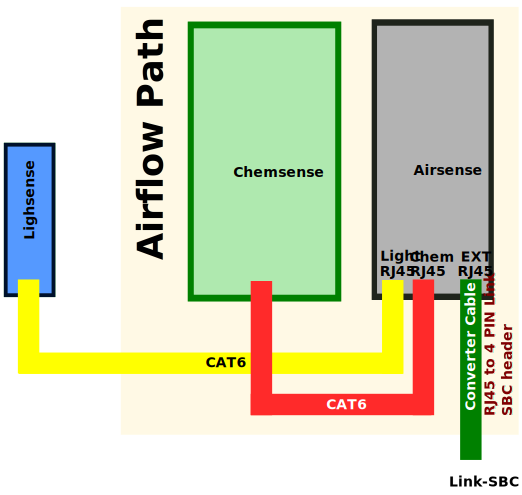
\includegraphics[width=4in]{link.pdf}
\caption{Connections between the sensor boards and interface to Link SBC}
\label{fig:physicalConnections}
\end{center}
\end{figure}


\newpage

\section{Data Transmission} \label{section:overall}

The data from the sensor boards is sent as a formatted unit of data -- a transmission
packet. A transmission packet is composed of several data sub-packets, each
of which carries information pertaining to the parameter listed in the sub-packet.
The data sub-packet, especially for additional sensors, rain gauge and soil moisture sensor, are described here.

\subsection{Data Sub-packets} \label{ssec:sub-pack}

The data segment of the transmission packet is further broken down into many
sub-packets. The sub-packet starts with a source identifier. One bit
validity field and seven bits ``length of the sub-packet'' field
are packed together as the next byte. The length field counts the number of
bytes following it which make up the sub-packet. The table below shows the organization
of a rain gauge sub-packet. 
\par
If the field is set to 1, it indicates a valid measurement/reading, 
and if the validity bit is set to 0 if the sensor represented in the sub-packet
is dead, disabled, unconnected, unresponsive or if data could not be collected
from the sensor in the time window. If the validity is 0, the particular invalid sub-packet is not packed into a transmission packet.

\subsubsection{Rain Gauge}
As shown in Table \ref{table:rain_subpacket}, sensor identifier of rain gauge is 0xFC, which is 252 in decimal, and if the data are valid, second byte will be 0x84, which means the sub-packet is valid and length of the sub-packet is 4 Bytes.


\begin{table}[H]
    \centering {
    \begin{tabular}{|c|c|c|c|}
        \hline
        \rowcolor{black!8}
        \textbf{Source ID} & \bf{1-bit Validity [0: invalid, 1: valid] | 7-bit Data Length} & \textbf{Data} \\
        \rowcolor{black!8}
        (1 Byte) & (1 Byte) & (2 Bytes) \\
        \hline
        0xFC & 0x84 (valid) & count of pendant event\\ 
        \hline
    \end{tabular}
    }
    \caption{Sub-packet for rain gauge}
    \label{table:rain_subpacket}
\end{table}


\subsubsection{Soil Moisture Sensor}
As shown in Table \ref{table:soil_subpacket}, sensor identifier of soil sensor is 0xFB, which is 251 in decimal,
and if the data are valid, second byte will be 0x84, which means the sub-packet is valid and length of the sub-packet is
6 Bytes.


\begin{table}[H]
    \centering {
    \begin{tabular}{|c|c|c|c|c|}
        \hline
        \rowcolor{black!8}
        \textbf{Source ID} & \bf{1-bit Validity | 7-bit Data Length} & \textbf{Data} \\
        \rowcolor{black!8}
        (1 Byte) & [0: invalid, 1: valid]  (1 Byte) & (6 Bytes) \\
        \hline
        \multirow{3}{*}{0xFB} & \multirow{3}{*}{0x86 (valid)} & Dielectric permittivity in Format 6 (2 Bytes) \\ \cline{3-3}
        & & Electric Conductivity in Format 6 (2 Bytes) \\ \cline{3-3}
        & & Temperature in Format 6 (2 Bytes) \\ \hline
    \end{tabular}
    }
    \caption{Sub-packet for rain gauge}
    \label{table:soil_subpacket}
\end{table}


\subsection{Data Formats}

The data sent in each sub-packet is encoded in one or more formats. Currently we define eight formats for various types of data including integers, bytes, and floating point numbers. 
Rain gauge data encoded as format 1, which is integers in range 0 to 65535, as shown in Table \ref{table:rain_format}.
Therefore the data of the rain gauge is an integer, and it means the count of pendant event inside the rain gauge. One event of the pendant means 0.01 in. (0.254 mm) of precipitation.
Soil sensor data is encoded as format 6, which is integers in range $-$127.99 to 127.99, as shown in Table \ref{table:rain_format}.
Therefore the data of the soil sensor are float point dielectric, conductivity, and temperature.
\\


\begin{table}[H]
    \centering {
    \begin{tabular}{|c|c|c|c|}
        \hline
        \rowcolor{black!8}
        \textbf{Format} & \textbf{Number of Bytes Used} & \textbf{Value Represented} & \textbf{Value Range} \\
        \hline
        1 & 2 & unsigned int\_16 input & 0 -- 65535 \\ %& MSByte LSByte\\
        6 & 2 & float input & [$-$127.99, 127.99] \\
        \hline
    \end{tabular}
    }
    \caption{Data format for rain gauge}
    \label{table:rain_format}
\end{table}

\clearpage
\section{Data Sub-Packet} \label{section:dataSub}

The data sub-packet consists of 32 "chunks" (30 sensors and 2 MAC addresses).  Each "chunk" follows one of seven formats.\\

%%%%%%%%%%%%%%%%%%%%

\subsection{Data Formats}

\begin{table}[H]
    \centering
    {\rowcolors{2}{black!12}{black!2}
    \begin{tabular}{|c c c c c c c|}
        \hline
        \textbf{Format} & \textbf{Byte 0} & \textbf{Byte 1} & \textbf{Byte 2} & \textbf{Byte 3} & \textbf{Byte 4} & \textbf{Byte 5}\\
        \hline
        \hline
        1 & (1 << 7) | 7-bit int & (neg << 7) | 7-bit frac. & - & - & - & -\\
        2 & 7 MSb & LSB & - & - & - & -\\
        3 & Addr5 & Addr4 & Addr3 & Addr2 & Addr1 & Addr0\\
        4 &
        \multirow{1}{8em}{(1 << 7) | (neg << 6) | (4-bit int << 2) | 2 MSb of frac.}
        & 8 LSb of frac. & - & - & - & -\\[4ex]
        5 & (neg << 6) | 6 MSb & 8 LSb & - & - & - & -\\
        6 &
        \multirow{1}{9em}{(1 << 7) | (neg << 6) | 6 MSb}
        & Middle 8 bits & 8 LSb & - & - & -\\[2ex]
        7 & First 8 "chunks" & 8 "chunks" & 8 "chunks" & Last 8 "chunks" & - & -\\
        \hline
    \end{tabular}
    }
    \caption{Data formats}
    \label{table:overall}
\end{table}

This version of the Waggle protocol does not use standard representations for floating point numbers.  Instead, the location of the decimal point is pre-determined (between the integer and fractional components, if applicable).\\

The most significant bit in byte 0 of formats 1, 4, and 6 means the data is already converted.  Formats 2 and 5 contain raw data.\\

Formats 1, 4, 5, and 6 contain a "negative" bit.  If this bit is 1, the value is negative.

%%%%%%%%%%%%%%%%%%%%

\subsection{Data "Chunks"}

The \textit{length} in each data "chunk" represents the number of bytes of sensor data.  The total "chunk" length is \textit{length} + 2.

\begin{table}[H]
    \centering
    {\rowcolors{2}{black!15}{black!8}
    \begin{tabular}{|c c c c|}
        \hline
        \textbf{Field} & \textbf{ID} & \textbf{Validity | Length} & \textbf{Data}\\
        \hline
        \hline
        Main MAC address & 0x00 & (1 << 7) | 0x06 & Table \ref{table:sensor1}\\
        TMP112 & 0x01 & (0/1 << 7) | 0x02 & Table \ref{table:sensor2}\\
        HTU21D & 0x02 & (0/1 << 7) | 0x04 & Table \ref{table:sensor3}\\
        GP2Y1010AU0F & 0x03 & (0/1 << 7) | 0x02 & Table \ref{table:sensor4}\\
        BMP180 & 0x04 & (0/1 << 7) | 0x05 & Table \ref{table:sensor5}\\
        PR103J2 & 0x05 & (0/1 << 7) | 0x02 & Table \ref{table:sensor6}\\
        TSL250RD & 0x06 & (0/1 << 7) | 0x02 & Table \ref{table:sensor6}\\
        MMA8452Q & 0x07 & (0/1 << 7) | 0x08 & Table \ref{table:sensor7}\\
        SPV1840LR5H-B & 0x08 & (0/1 << 7) | 0x02 & Table \ref{table:sensor8}\\
        TSYS01 & 0x09 & (0/1 << 7) | 0x02 & Table \ref{table:sensor9}\\
        HMC5883L & 0x0A & (0/1 << 7) | 0x06 & Table \ref{table:sensor10}\\
        HIH6130 & 0x0B & (0/1 << 7) | 0x04 & Table \ref{table:sensor3}\\
        APDS-9006-020 & 0x0C & (0/1 << 7) | 0x02 & Table \ref{table:sensor6}\\
        TSL260RD & 0x0D & (0/1 << 7) | 0x02 & Table \ref{table:sensor6}\\
        TSL250RD & 0x0E & (0/1 << 7) | 0x02 & Table \ref{table:sensor6}\\
        MLX75305 & 0x0F & (0/1 << 7) | 0x02 & Table \ref{table:sensor6}\\
        ML8511 & 0x10 & (0/1 << 7) | 0x02 & Table \ref{table:sensor6}\\
        D6T & 0x11 & (0/1 << 7) | 0x22 & Table \ref{table:sensor11}\\
        MLX90614 & 0x12 & (0/1 << 7) | 0x02 & Table \ref{table:sensor2}\\
        TMP421 & 0x13 & (0/1 << 7) | 0x02 & Table \ref{table:sensor2}\\
        SPV1840LR5H-B & 0x14 & (0/1 << 7) | 0x02 & Table \ref{table:sensor8}\\
        Total reducing gases & 0x15 & (0/1 << 7) | 0x02 & Table \ref{table:sensor12}\\
        Ethanol & 0x16 & (0/1 << 7) | 0x02 & Table \ref{table:sensor12}\\
        Nitrogen dioxide & 0x17 & (0/1 << 7) | 0x02 & Table \ref{table:sensor12}\\
        Ozone & 0x18 & (0/1 << 7) | 0x02 & Table \ref{table:sensor12}\\
        Hydrogen sulphide & 0x19 & (0/1 << 7) | 0x02 & Table \ref{table:sensor12}\\
        Total oxidizing gases & 0x1A & (0/1 << 7) | 0x02 & Table \ref{table:sensor12}\\
        Carbon monoxide & 0x1B & (0/1 << 7) | 0x02 & Table \ref{table:sensor12}\\
        Sulfur dioxide & 0x1C & (0/1 << 7) | 0x02 & Table \ref{table:sensor12}\\
        Sensirion & 0x1D & (0/1 << 7) | 0x04 & Table \ref{table:sensor3}\\
        Bosh & 0x1E & (0/1 << 7) | 0x03 & Table \ref{table:sensor13}\\
        Intel MAC address & 0x1F & (1 << 7) | 0x06 & Table \ref{table:sensor1}\\
        Sensor status (health) & 0xFE & (1 << 7) | 0x04 & Table \ref{table:sensor14}\\
        \hline
    \end{tabular}
    }
    \caption{Data sub-packet structure (each row is a "chunk")}
    \label{table:dataChunk}
\end{table}

\begin{table}[H]
    \centering
    {\rowcolors{2}{black!12}{black!2}
    \begin{tabular}{|c c c c c c|}
        \hline
        \textbf{Byte 0} & \textbf{Byte 1} & \textbf{Byte 2} & \textbf{Byte 3} & \textbf{Byte 4} & \textbf{Byte 5}\\
        \hline
        \hline
        Address 5 & Address 4 & Address 3 & Address 2 & Address 1 & Address 0\\
        \multicolumn{6}{|c|}{Format 3}\\
        \hline
    \end{tabular}
    }
    \caption{MAC address}
    \label{table:sensor1}
\end{table}

\begin{table}[H]
    \centering
    {\rowcolors{2}{black!12}{black!2}
    \begin{tabular}{|c c|}
        \hline
        \textbf{Byte 0} & \textbf{Byte 1}\\
        \hline
        \hline
        \multicolumn{2}{|c|}{Temperature}\\
        \multicolumn{2}{|c|}{Format 1}\\
        \hline
    \end{tabular}
    }
    \caption{Sensor data}
    \label{table:sensor2}
\end{table}

\begin{table}[H]
    \centering
    {\rowcolors{2}{black!12}{black!2}
    \begin{tabular}{|c c c c|}
        \hline
        \textbf{Byte 0} & \textbf{Byte 1} & \textbf{Byte 2} & \textbf{Byte 3}\\
        \hline
        \hline
        \multicolumn{2}{|c|}{Temperature} & \multicolumn{2}{|c|}{Humidity}\\
        \multicolumn{2}{|c|}{Format 1} & \multicolumn{2}{|c|}{Format 1}\\
        \hline
    \end{tabular}
    }
    \caption{Sensor data}
    \label{table:sensor3}
\end{table}

\begin{table}[H]
    \centering
    {\rowcolors{2}{black!12}{black!2}
    \begin{tabular}{|c c|}
        \hline
        \textbf{Byte 0} & \textbf{Byte 1}\\
        \hline
        \hline
        \multicolumn{2}{|c|}{Dust}\\
        \multicolumn{2}{|c|}{Format 2}\\
        \hline
    \end{tabular}
    }
    \caption{Sensor data}
    \label{table:sensor4}
\end{table}

\begin{table}[H]
    \centering
    {\rowcolors{2}{black!12}{black!2}
    \begin{tabular}{|c c c c c|}
        \hline
        \textbf{Byte 0} & \textbf{Byte 1} & \textbf{Byte 2} & \textbf{Byte 3} & \textbf{Byte 4}\\
        \hline
        \hline
        \multicolumn{2}{|c|}{Temperature} & \multicolumn{3}{|c|}{Atmospheric pressure}\\
        \multicolumn{2}{|c|}{Format 1} & \multicolumn{3}{|c|}{Format 6}\\
        \hline
    \end{tabular}
    }
    \caption{Sensor data}
    \label{table:sensor5}
\end{table}

\begin{table}[H]
    \centering
    {\rowcolors{2}{black!12}{black!2}
    \begin{tabular}{|c c|}
        \hline
        \textbf{Byte 0} & \textbf{Byte 1}\\
        \hline
        \hline
        \multicolumn{2}{|c|}{Light}\\
        \multicolumn{2}{|c|}{Format 2}\\
        \hline
    \end{tabular}
    }
    \caption{Sensor data}
    \label{table:sensor6}
\end{table}

\begin{table}[H]
    \centering
    {\rowcolors{2}{black!12}{black!2}
    \begin{tabular}{|c c c c c c c c|}
        \hline
        \textbf{Byte 0} & \textbf{Byte 1}  & \textbf{Byte 2} & \textbf{Byte 3} & \textbf{Byte 4} & \textbf{Byte 5} & \textbf{Byte 6} & \textbf{Byte 7}\\
        \hline
        \hline
        \multicolumn{2}{|c|}{Acceleration X} & \multicolumn{2}{|c|}{Acceleration Y}  & \multicolumn{2}{|c|}{Acceleration Z} & \multicolumn{2}{|c|}{RMS}\\
        \multicolumn{2}{|c|}{Format 1} & \multicolumn{2}{|c|}{Format 1}  & \multicolumn{2}{|c|}{Format 1} & \multicolumn{2}{|c|}{Format 1}\\
        \hline
    \end{tabular}
    }
    \caption{Sensor data}
    \label{table:sensor7}
\end{table}

\begin{table}[H]
    \centering
    {\rowcolors{2}{black!12}{black!2}
    \begin{tabular}{|c c|}
        \hline
        \textbf{Byte 0} & \textbf{Byte 1}\\
        \hline
        \hline
        \multicolumn{2}{|c|}{Sound pressure}\\
        \multicolumn{2}{|c|}{Format 2}\\
        \hline
    \end{tabular}
    }
    \caption{Sensor data}
    \label{table:sensor8}
\end{table}

\begin{table}[H]
    \centering
    {\rowcolors{2}{black!12}{black!2}
    \begin{tabular}{|c c|}
        \hline
        \textbf{Byte 0} & \textbf{Byte 1}\\
        \hline
        \hline
        \multicolumn{2}{|c|}{Temperature}\\
        \multicolumn{2}{|c|}{Format 2}\\
        \hline
    \end{tabular}
    }
    \caption{Sensor data}
    \label{table:sensor9}
\end{table}

\begin{table}[H]
    \centering
    {\rowcolors{2}{black!12}{black!2}
    \begin{tabular}{|c c c c c c|}
        \hline
        \textbf{Byte 0} & \textbf{Byte 1}  & \textbf{Byte 2} & \textbf{Byte 3} & \textbf{Byte 4} & \textbf{Byte 5}\\
        \hline
        \hline
        \multicolumn{2}{|c|}{Magnetic X} & \multicolumn{2}{|c|}{Magnetic Y}  & \multicolumn{2}{|c|}{Magnetic Z}\\
        \multicolumn{2}{|c|}{Format 4} & \multicolumn{2}{|c|}{Format 4}  & \multicolumn{2}{|c|}{Format 4}\\
        \hline
    \end{tabular}
    }
    \caption{Sensor data}
    \label{table:sensor10}
\end{table}

\begin{table}[H]
    \centering
    {\rowcolors{2}{black!12}{black!2}
    \begin{tabular}{|c c c c c|}
        \hline
        \textbf{Byte 0} & \textbf{Byte 1} & \textbf{...} & \textbf{Byte 32} & \textbf{Byte 33}\\
        \hline
        \hline
        \multicolumn{2}{|c|}{Temperature} & Temperature & \multicolumn{2}{|c|}{Temperature}\\
        \multicolumn{2}{|c|}{Format 1} & Format 1 & \multicolumn{2}{|c|}{Format 1}\\
        \hline
    \end{tabular}
    }
    \caption{Sensor data}
    \label{table:sensor11}
\end{table}

\begin{table}[H]
    \centering
    {\rowcolors{2}{black!12}{black!2}
    \begin{tabular}{|c c|}
        \hline
        \textbf{Byte 0} & \textbf{Byte 1}\\
        \hline
        \hline
        \multicolumn{2}{|c|}{Gas concentration}\\
        \multicolumn{2}{|c|}{Format 2}\\
        \hline
    \end{tabular}
    }
    \caption{Sensor data}
    \label{table:sensor12}
\end{table}

\begin{table}[H]
    \centering
    {\rowcolors{2}{black!12}{black!2}
    \begin{tabular}{|c c c|}
        \hline
        \textbf{Byte 0} & \textbf{Byte 1} & \textbf{Byte 2}\\
        \hline
        \hline
        \multicolumn{3}{|c|}{Atmospheric pressure}\\
        \multicolumn{3}{|c|}{Format 6}\\
        \hline
    \end{tabular}
    }
    \caption{Sensor data}
    \label{table:sensor13}
\end{table}

\begin{table}[H]
    \centering
    {\rowcolors{2}{black!12}{black!2}
    \begin{tabular}{|c c c c|}
        \hline
        \textbf{Byte 0} & \textbf{Byte 1} & \textbf{Byte 2}  & \textbf{Byte 3}\\
        \hline
        \hline
        \multicolumn{4}{|c|}{Health status (1 bit per "chunk")}\\
        \multicolumn{4}{|c|}{Format 7}\\
        \hline
    \end{tabular}
    }
    \caption{Sensor status (health)}
    \label{table:sensor14}
\end{table}

%%%%%%%%%%%%%%%%%%%%
\newpage
\section{Sub-packets}

As shortly explained in document section \ref{ssec:sub-pack}, data sub-packets are generated depending on its designated data format and length. The first byte of the sub-packet is sensor ID for each parameter, and the second byte means validity of the packet and length of the sensor data. The packet validity is initially 0, and it will be changed to 1 when each sub-packet gets sensor value from sensor. And after a transmission packet is trasmitted, the validity becomes 0 again. The form of sub-packet is shown below.

\begin{table}[H]
\centering
\begin{tabular}{|c|c|c|}
\hline
% column1a & column2a \\
\noalign{\hrule height 2pt}
\multicolumn{1}{!{\vrule width 2pt}c!{\vrule width 1pt}}{Source ID} &
\multicolumn{1}{!{\vrule width 2pt}c!{\vrule width 1pt}}{1-bit Validity | 7-bits Sensor Data Length} &
\multicolumn{1}{!{\vrule width 2pt}c!{\vrule width 1pt}}{Data} \\
\noalign{\hrule height 2pt}
One Byte & One Byte & up to 127 Bytes \\
\hline
\end{tabular}
\end{table}


\subsection{Parameters}

The sensor boards output a set of parameters which are identified by a unique ID. Each parameter
has a set of values associated with it which are encoded in an appropriate data format. The table
below lists the various parameters produced by the sensor boards, the unique source ID used to identify them, the values produced by them and the format in which the value is encoded.


\begin{center}
\rowcolors{2}{white}{black!5}
\begin{longtable}{|l|c|l|}
\caption{Data sub-packet structure (each row is a "chunk")} \label{tab:dataChunk} \\

\hline \rowcolor{white} \multicolumn{1}{|c|}{\textbf{Parameter}} & \multicolumn{1}{c|}{\textbf{Source ID}} & \multicolumn{1}{c|}{\textbf{Values and Formats}} \\ \hline
\endfirsthead

\multicolumn{3}{c}%
{{\bfseries \tablename\ \thetable{} -- continued from previous page}} \\
\hline \rowcolor{white} \multicolumn{1}{|c|}{\textbf{Parameter}} & \multicolumn{1}{c|}{\textbf{Source ID}} & \multicolumn{1}{c|}{\textbf{Values and Formats}} \\ \hline 
\endhead

\hline \rowcolor{white} \multicolumn{3}{|r|}{{Continued on next page}} \\ \hline
\endfoot

\hline \hline
\endlastfoot

     \hline \rowcolor{white} \multicolumn{3}{|c|}{{Airsense board}} \\ \hline
        Airsense/Lightsense MAC address & 0x00 & MAC Address -- Format 3 \\
        TMP112 & 0x01 & Temperature -- Format 6\\
        HTU21D & 0x02 & Temperature and Humidity -- Format 6\\
        HIH4030 & 0x03 & Humidity -- Format 1 \\
        BMP180 & 0x04 & Temperature -- Format 6 \& Pressure -- Format 4\\
        PR103J2 & 0x05 & Temperature -- Format 1\\
        TSL250RD & 0x06 & Visible Light -- Format 1\\
        MMA8452Q & 0x07 & Three Accelerations and Vibration -- Format 6\\
        SPV1840LR5H-B & 0x08 & RMS Sound Level -- Format 1\\
        TSYS01 & 0x09 & Temperature -- Format 6\\
     \hline \rowcolor{white} \multicolumn{3}{|c|}{{Lightsense board}} \\ \hline
        HMC5883L & 0x0A & Three Magnetic Fields -- Format 8\\
        HIH6130 & 0x0B & Temperature and Humidity -- Format 6\\
        APDS-9006-020 & 0x0C & Visible Light -- Format 1\\
        TSL260RD & 0x0D & IR Light -- Format 1\\
        TSL250RD & 0x0E & Visible Light -- Format 1\\
        MLX75305 & 0x0F & Light -- Format 1\\
        ML8511 & 0x10 & Light -- Format 1\\
        MLX90614 & 0x12 & Temperature -- Format 6\\
        TMP421 & 0x13 & Temperature -- Format 6\\
%         Lightsense MAC address & 0x14 & MAC Address -- Format 3 \\
     \hline \rowcolor{white} \multicolumn{3}{|c|}{{Chemsense board}} \\ \hline
        Total reducing gases & 0x15 & Raw Concentration -- Format 5\\
        Nitrogen dioxide & 0x17 & Raw Concentration -- Format 5\\
        Ozone & 0x18 & Raw Concentration -- Format 5\\
        Hydrogen sulphide & 0x19 & Raw Concentration -- Format 5\\
        Total oxidizing gases & 0x1A & Raw Concentration -- Format 5\\
        Carbon monoxide & 0x1B & Raw Concentration -- Format 5\\
        Sulfur dioxide & 0x1C & Raw Concentration -- Format 5\\
        SHT25 & 0x1D & Temperature \& Humidity -- Format 2\\
        LPS25H & 0x1E & Temperature -- Format 2 \& Pressure -- Format 4\\
        Si1145 & 0x1F & UV intensity -- Format 1\\
        Chemsense MAC address & 0x20 & MAC Address -- Format 3\\
        CO ADC temp & 0x21 & ADC temperature -- Format 2\\
        IAQ IRR ADC temp & 0x22 & ADC temperature -- Format 2\\
        O3 NO2 ADC temp & 0x23 & ADC temperature -- Format 2\\
        SO2 H2S ADC temp & 0x24 & ADC temperature -- Format 2\\
        CO LMP temp & 0x25 & ADC temperature -- Format 2\\
        Accelerometer & 0x26 & Three Accelerations -- Format 2 \& Vibration -- Format 4\\
        Gyro & 0x27 & Three Orientation -- Format 2 \& Orientation Index -- Format 4\\
     \hline \rowcolor{white} \multicolumn{3}{|c|}{{Alpha sensor}} \\ \hline
        Histogram & 0x28 & Various particle information including Particulate Matter\\
        Firmware & 0x29 & Firmware version  -- unsigned integer\\
        Configuration A & 0x30 & Sensor Configuration packet A -- unsigned integer\\
        Configuration B & 0x31 & Sensor Configuration packet B -- unsigned integer\\
        Configuration C & 0x32 & Sensor Configuration packet C -- unsigned integer\\
        Configuration D & 0x33 & Sensor Configuration packet D -- unsigned integer\\
\end{longtable}
\end{center}


Each parameter and its values are composed into a sub-packet based on
the format described in document section \ref{ssec:sub-pack}.
In the case of parameters with 2 or more values, the encoded values are
arranged in the sub-packets sequentially. The context of each parameter,
its utility and the arrangement of its values is described below. In all
the tables below, the validity bit is set to 1. The parameter descriptions
below are aggregated based on the sensor-board they are situated on -
Airsense, Lightsense and Chemsense.
% document subsections \ref{ssec:first} to \ref{ssec:last}.

\subsection{Airsense:}
\subsubsection{ Airsense/Lightsense MAC address} \label{ssec:first}

This is a six byte ID that uniquely identifies each Airsense board. This MAC address is also applied to each Lightsense board which has the same board number. The ID is provided by a DS2401 1-Wire DSN chip. The 1-byte family ID and CRC provided by the DSN chip are omitted, and the rest six bytes are used as the Unique ID. The Unique ID uses Format 3 for encoding and the arrangement is listed below.

\begin{table}[H]
\centering
\begin{tabular}{|c|c|c|}
\hline
% column1a & column2a \\
\noalign{\hrule height 2pt}
\multicolumn{1}{!{\vrule width 2pt}c!{\vrule width 1pt}}{0x00} &
\multicolumn{1}{!{\vrule width 2pt}c!{\vrule width 1pt}}{0x86} &
\multicolumn{1}{!{\vrule width 2pt}c!{\vrule width 1pt}}{ID in Format 3}\\
\noalign{\hrule height 2pt}
Byte[0] & Byte[1] & Bytes[2 -- 7]\\
\hline
\end{tabular}
\end{table}

\subsubsection{ TMP112}

TMP112 is a digital temperature sensor, which provides the temperature values
in centigrade.

\begin{table}[H]
\centering
\begin{tabular}{|c|c|c|c|}
\hline
% column1a & column2a \\
\noalign{\hrule height 2pt}
\multicolumn{1}{!{\vrule width 2pt}c!{\vrule width 1pt}}{0x01} &
\multicolumn{1}{!{\vrule width 2pt}c!{\vrule width 1pt}}{0x82} &
\multicolumn{1}{!{\vrule width 2pt}c!{\vrule width 1pt}}{Temperature in Format 6} \\
\noalign{\hrule height 2pt}
Byte[0] & Byte[1] & Bytes[2 -- 3] \\
\hline
\end{tabular}
\end{table}


\begin{table}[H]
\centering
\begin{tabular}{|c|c|c|c|}
\hline
% column1a & column2a \\
\noalign{\hrule height 2pt}
\multicolumn{1}{!{\vrule width 2pt}c!{\vrule width 1pt}}{Value} &
\multicolumn{1}{!{\vrule width 2pt}c!{\vrule width 1pt}}{Board Output} &
\multicolumn{1}{!{\vrule width 2pt}c!{\vrule width 1pt}}{Post-Processing Mode} &
\multicolumn{1}{!{\vrule width 2pt}c!{\vrule width 1pt}}{Post-processed Output} \\
\noalign{\hrule height 2pt}
Temperature & $^{\circ}$C & None & None \\
\hline
\end{tabular}
\end{table}

\subsubsection{ HTU21D}
HTU21D is a digital temperature and humidity sensor, which provides
relative humidity value (\%RH) and temperature value in centigrade.

\begin{table}[H]
\centering
\begin{tabular}{|c|c|c|c|c|}
\hline
% column1a & column2a \\
\noalign{\hrule height 2pt}
\multicolumn{1}{!{\vrule width 2pt}c!{\vrule width 1pt}}{0x02} &
\multicolumn{1}{!{\vrule width 2pt}c!{\vrule width 1pt}}{0x84} &
\multicolumn{1}{!{\vrule width 2pt}c!{\vrule width 1pt}}{Temperature in Format 6}&
\multicolumn{1}{!{\vrule width 2pt}c!{\vrule width 1pt}}{\%RH in Format 6}\\
\noalign{\hrule height 2pt}
Byte[0] & Byte[1] & Bytes[2 -- 3]  & Bytes [4 -- 5]\\
\hline
\end{tabular}
\end{table}

\begin{table}[H]
\centering
\begin{tabular}{|c|c|c|c|}
\hline
% column1a & column2a \\
\noalign{\hrule height 2pt}
\multicolumn{1}{!{\vrule width 2pt}c!{\vrule width 1pt}}{Value} &
\multicolumn{1}{!{\vrule width 2pt}c!{\vrule width 1pt}}{Board Output} &
\multicolumn{1}{!{\vrule width 2pt}c!{\vrule width 1pt}}{Post-Processing Mode} &
\multicolumn{1}{!{\vrule width 2pt}c!{\vrule width 1pt}}{Post-processed Output} \\
\noalign{\hrule height 2pt}
Temperature & $^{\circ}$C & None & None \\
\hline
Relative Humidity & \%RH & None & None \\
\hline
\end{tabular}
\end{table}

\subsubsection{ HIH4030}

HIH4030 is an analog humidity sensor, which provides an analog voltage representative
of the relative humidity. The analog voltage is converted and packed into Format 1 using
a 10-bit ADC.

\begin{table}[H]
\centering
\begin{tabular}{|c|c|c|c|}
\hline
% column1a & column2a \\
\noalign{\hrule height 2pt}
\multicolumn{1}{!{\vrule width 2pt}c!{\vrule width 1pt}}{0x03} &
\multicolumn{1}{!{\vrule width 2pt}c!{\vrule width 1pt}}{0x82} &
\multicolumn{1}{!{\vrule width 2pt}c!{\vrule width 1pt}}{RH in Format 1}\\
\noalign{\hrule height 2pt}
Byte[0] & Byte[1] & Bytes[2 -- 3]\\
\hline
\end{tabular}
\end{table}


\begin{table}[H]
\centering
\begin{tabular}{|c|c|c|c|}
\hline
% column1a & column2a \\
\noalign{\hrule height 2pt}
\multicolumn{1}{!{\vrule width 2pt}c!{\vrule width 1pt}}{Value} &
\multicolumn{1}{!{\vrule width 2pt}c!{\vrule width 1pt}}{Board Output} &
\multicolumn{1}{!{\vrule width 2pt}c!{\vrule width 1pt}}{Post-Processing Mode} &
\multicolumn{1}{!{\vrule width 2pt}c!{\vrule width 1pt}}{Post-processed Output} \\
\noalign{\hrule height 2pt}
Relative Humidity & raw integer & Bulk Curve Fitting & \%RH \\
\hline
\end{tabular}
\end{table}


\subsubsection{ BMP180}

BMP180 is an digital temperature and barometric pressure sensor,
which provides temperature in centigrade and pressure in hectopascals.

\begin{table}[H]
\centering
\begin{tabular}{|c|c|c|c|c|}
\hline
% column1a & column2a \\
\noalign{\hrule height 2pt}
\multicolumn{1}{!{\vrule width 2pt}c!{\vrule width 1pt}}{0x04} &
\multicolumn{1}{!{\vrule width 2pt}c!{\vrule width 1pt}}{0x85} &
\multicolumn{1}{!{\vrule width 2pt}c!{\vrule width 1pt}}{Temperature in Format 6}&
\multicolumn{1}{!{\vrule width 2pt}c!{\vrule width 1pt}}{Pressure in Format 4}\\
\noalign{\hrule height 2pt}
Byte[0] & Byte[1] & Bytes[2 -- 3] & Bytes [4 -- 6]\\
\hline
\end{tabular}
\end{table}



\begin{table}[H]
\centering
\begin{tabular}{|c|c|c|c|}
\hline
% column1a & column2a \\
\noalign{\hrule height 2pt}
\multicolumn{1}{!{\vrule width 2pt}c!{\vrule width 1pt}}{Value} &
\multicolumn{1}{!{\vrule width 2pt}c!{\vrule width 1pt}}{Board Output} &
\multicolumn{1}{!{\vrule width 2pt}c!{\vrule width 1pt}}{Post-Processing Mode} &
\multicolumn{1}{!{\vrule width 2pt}c!{\vrule width 1pt}}{Post-processed Output} \\
\noalign{\hrule height 2pt}
Temperature & $^{\circ}$C & None & None \\
\hline
Atmospheric Pressure & hPa & None & None \\
\hline
\end{tabular}
\end{table}

\subsubsection{ PR103J2}

PR103J2 is an analog temperature sensor whose resistance changes with change in temperature.
The sensor is implemented in a voltage divider circuit, and the center-tap voltage is converted and packed into Format 1 using a 10-bit ADC.

\begin{table}[H]
\centering
\begin{tabular}{|c|c|c|c|}
\hline
% column1a & column2a \\
\noalign{\hrule height 2pt}
\multicolumn{1}{!{\vrule width 2pt}c!{\vrule width 1pt}}{0x05} &
\multicolumn{1}{!{\vrule width 2pt}c!{\vrule width 1pt}}{0x82} &
\multicolumn{1}{!{\vrule width 2pt}c!{\vrule width 1pt}}{Temperature in Format 1}\\
\noalign{\hrule height 2pt}
Byte[0] & Byte[1] & Bytes[2 -- 3]\\
\hline
\end{tabular}
\end{table}

\begin{table}[H]
\centering
\begin{tabular}{|c|c|c|c|}
\hline
% column1a & column2a \\
\noalign{\hrule height 2pt}
\multicolumn{1}{!{\vrule width 2pt}c!{\vrule width 1pt}}{Value} &
\multicolumn{1}{!{\vrule width 2pt}c!{\vrule width 1pt}}{Board Output} &
\multicolumn{1}{!{\vrule width 2pt}c!{\vrule width 1pt}}{Post-Processing Mode} &
\multicolumn{1}{!{\vrule width 2pt}c!{\vrule width 1pt}}{Post-processed Output} \\
\noalign{\hrule height 2pt}
Temperature & raw integer & Bulk Curve Fitting & $^{\circ}$C \\
\hline
\end{tabular}
\end{table}

\subsubsection{ TSL250RD}

TSL250RD is an analog visible light sensor that produces an analog voltage that is
representative of the irradiance measured in $\mu$W/cm$^2$. The output voltage of the sensor
is converted and packed into Format 1 using a 10-bit ADC.

\begin{table}[H]
\centering
\begin{tabular}{|c|c|c|c|}
\hline
% column1a & column2a \\
\noalign{\hrule height 2pt}
\multicolumn{1}{!{\vrule width 2pt}c!{\vrule width 1pt}}{0x06} &
\multicolumn{1}{!{\vrule width 2pt}c!{\vrule width 1pt}}{0x82} &
\multicolumn{1}{!{\vrule width 2pt}c!{\vrule width 1pt}}{Light intensity in Format 1}\\
\noalign{\hrule height 2pt}
Byte[0] & Byte[1] & Bytes[2 -- 3]\\
\hline
\end{tabular}
\end{table}

\begin{table}[H]
\centering
\begin{tabular}{|c|c|c|c|}
\hline
% column1a & column2a \\
\noalign{\hrule height 2pt}
\multicolumn{1}{!{\vrule width 2pt}c!{\vrule width 1pt}}{Value} &
\multicolumn{1}{!{\vrule width 2pt}c!{\vrule width 1pt}}{Board Output} &
\multicolumn{1}{!{\vrule width 2pt}c!{\vrule width 1pt}}{Post-Processing Mode} &
\multicolumn{1}{!{\vrule width 2pt}c!{\vrule width 1pt}}{Post-processed Output} \\
\noalign{\hrule height 2pt}
Light Intensity & raw integer & Bulk Curve Fitting & $\mu$W/cm$^2$ \\
\hline
\end{tabular}
\end{table}


\subsubsection{ MMA8452Q}

MMA8452Q is a digital three-axis accelerometer. The accelerations in three orthogonal directions,
x, y and z, as a multiple of acceleration due to gravity (g) are obtained from the sensor,
and a vibration value (represented as multiple of g) is calculated using high-frequency
time series data from the three axis.

\begin{table}[H]
\centering
\begin{tabular}{|c|c|c|c|c|c|}
\hline
% column1a & column2a \\
\noalign{\hrule height 2pt}
\multicolumn{1}{!{\vrule width 2pt}c!{\vrule width 1pt}}{0x07} &
\multicolumn{1}{!{\vrule width 2pt}c!{\vrule width 1pt}}{0x88} &
\multicolumn{1}{!{\vrule width 2pt}c!{\vrule width 1pt}}{Acc. X in Format 6}&
\multicolumn{1}{!{\vrule width 2pt}c!{\vrule width 1pt}}{Acc. Y in Format 6}&
\multicolumn{1}{!{\vrule width 2pt}c!{\vrule width 1pt}}{Acc. Z in Format 6}&
\multicolumn{1}{!{\vrule width 2pt}c!{\vrule width 1pt}}{Vibration in Format 6}\\
\noalign{\hrule height 2pt}
Byte[0] & Byte[1] & Bytes[2 -- 3] & Bytes[4 -- 5] & Bytes[6 -- 7] & Bytes[8 -- 9]\\
\hline
\end{tabular}
\end{table}



\begin{table}[H]
\centering
\begin{tabular}{|c|c|c|c|}
\hline
% column1a & column2a \\
\noalign{\hrule height 2pt}
\multicolumn{1}{!{\vrule width 2pt}c!{\vrule width 1pt}}{Value} &
\multicolumn{1}{!{\vrule width 2pt}c!{\vrule width 1pt}}{Board Output} &
\multicolumn{1}{!{\vrule width 2pt}c!{\vrule width 1pt}}{Post-Processing Mode} &
\multicolumn{1}{!{\vrule width 2pt}c!{\vrule width 1pt}}{Post-processed Output} \\
\noalign{\hrule height 2pt}
Acc. X & g & none & none \\
\hline
Acc. Y & g & none & none \\
\hline
Acc. Z & g & none & none \\
\hline
Vibration & g & none & none \\
\hline
\end{tabular}
\end{table}

\subsubsection{ SPV1840LR5H-B}

SPV1840LR5H is a MEMS microphone that is sampled at high frequency to obtain
the peaks and calculate the sound intensity for a time window. The raw calculated
intensity is represented as a 16-bit integer value using Format 1.

\begin{table}[H]
\centering
\begin{tabular}{|c|c|c|c|c|c|}
\hline
% column1a & column2a \\
\noalign{\hrule height 2pt}
\multicolumn{1}{!{\vrule width 2pt}c!{\vrule width 1pt}}{0x08} &
\multicolumn{1}{!{\vrule width 2pt}c!{\vrule width 1pt}}{0x82} &
\multicolumn{1}{!{\vrule width 2pt}c!{\vrule width 1pt}}{Sound Intensity in Format 1}\\
\noalign{\hrule height 2pt}
Byte[0] & Byte[1] & Bytes[2 -- 3]\\
\hline
\end{tabular}
\end{table}


\begin{table}[H]
\centering
\begin{tabular}{|c|c|c|c|}
\hline
% column1a & column2a \\
\noalign{\hrule height 2pt}
\multicolumn{1}{!{\vrule width 2pt}c!{\vrule width 1pt}}{Value} &
\multicolumn{1}{!{\vrule width 2pt}c!{\vrule width 1pt}}{Board Output} &
\multicolumn{1}{!{\vrule width 2pt}c!{\vrule width 1pt}}{Post-Processing Mode} &
\multicolumn{1}{!{\vrule width 2pt}c!{\vrule width 1pt}}{Post-processed Output} \\
\noalign{\hrule height 2pt}
Sound Intensity & raw integer & Bulk Curve Fitting & dB \\
\hline
\end{tabular}
\end{table}


\subsubsection{ TSYS01}

TSYS01 is a digital temperature sensor, which provides the temperature values
in centigrade.

\begin{table}[H]
\centering
\begin{tabular}{|c|c|c|c|}
\hline
% column1a & column2a \\
\noalign{\hrule height 2pt}
\multicolumn{1}{!{\vrule width 2pt}c!{\vrule width 1pt}}{0x09} &
\multicolumn{1}{!{\vrule width 2pt}c!{\vrule width 1pt}}{0x82} &
\multicolumn{1}{!{\vrule width 2pt}c!{\vrule width 1pt}}{Temperature in Format 6} \\
\noalign{\hrule height 2pt}
Byte[0] & Byte[1] & Bytes[2 -- 3]\\
\hline
\end{tabular}
\end{table}

\begin{table}[H]
\centering
\begin{tabular}{|c|c|c|c|}
\hline
% column1a & column2a \\
\noalign{\hrule height 2pt}
\multicolumn{1}{!{\vrule width 2pt}c!{\vrule width 1pt}}{Value} &
\multicolumn{1}{!{\vrule width 2pt}c!{\vrule width 1pt}}{Board Output} &
\multicolumn{1}{!{\vrule width 2pt}c!{\vrule width 1pt}}{Post-Processing Mode} &
\multicolumn{1}{!{\vrule width 2pt}c!{\vrule width 1pt}}{Post-processed Output} \\
\noalign{\hrule height 2pt}
Temperature & $^{\circ}$C & None & None \\
\hline
\end{tabular}
\end{table}


\subsection{Lightsense:}
\subsubsection{ HMC5883L}


HMC5883L is a digital three-axis magnetometer. The magnetic field strengths in three orthogonal directions,
x, y and z are obtained from the sensor.

\begin{table}[H]
\centering
\begin{tabular}{|c|c|c|c|c|}
\hline
% column1a & column2a \\
\noalign{\hrule height 2pt}
\multicolumn{1}{!{\vrule width 2pt}c!{\vrule width 1pt}}{0x0A} &
\multicolumn{1}{!{\vrule width 2pt}c!{\vrule width 1pt}}{0x88} &
\multicolumn{1}{!{\vrule width 2pt}c!{\vrule width 1pt}}{Field strength X in Format 8}&
\multicolumn{1}{!{\vrule width 2pt}c!{\vrule width 1pt}}{Field strength Y in Format 8}&
\multicolumn{1}{!{\vrule width 2pt}c!{\vrule width 1pt}}{Field strength Z in Format 8}\\
\noalign{\hrule height 2pt}
Byte[0] & Byte[1] & Bytes[2 -- 3] & Bytes[4 -- 5] & Bytes[6 -- 7]\\
\hline
\end{tabular}
\end{table}

\begin{table}[H]
\centering
\begin{tabular}{|c|c|c|c|}
\hline
% column1a & column2a \\
\noalign{\hrule height 2pt}
\multicolumn{1}{!{\vrule width 2pt}c!{\vrule width 1pt}}{Value} &
\multicolumn{1}{!{\vrule width 2pt}c!{\vrule width 1pt}}{Board Output} &
\multicolumn{1}{!{\vrule width 2pt}c!{\vrule width 1pt}}{Post-Processing Mode} &
\multicolumn{1}{!{\vrule width 2pt}c!{\vrule width 1pt}}{Post-processed Output} \\
\noalign{\hrule height 2pt}
Mag. Field X & Gauss & none & none \\
\hline
Mag. Field Y & Gauss & none & none \\
\hline
Mag. Field Z & Gauss & none & none \\
\hline
\end{tabular}
\end{table}

\subsubsection{ HIH6130}

HIH6130 is a digital temperature and humidity sensor, which provides
relative humidity value (\%RH) and temperature value in centigrade.

\begin{table}[H]
\centering
\begin{tabular}{|c|c|c|c|c|}
\hline
% column1a & column2a \\
\noalign{\hrule height 2pt}
\multicolumn{1}{!{\vrule width 2pt}c!{\vrule width 1pt}}{0x0B} &
\multicolumn{1}{!{\vrule width 2pt}c!{\vrule width 1pt}}{0x84} &
\multicolumn{1}{!{\vrule width 2pt}c!{\vrule width 1pt}}{Temperature in Format 6}&
\multicolumn{1}{!{\vrule width 2pt}c!{\vrule width 1pt}}{\%RH in Format 6}\\
\noalign{\hrule height 2pt}
Byte[0] & Byte[1] & Bytes[2 -- 3] & Bytes[4 -- 5]\\
\hline
\end{tabular}
\end{table}

\begin{table}[H]
\centering
\begin{tabular}{|c|c|c|c|}
\hline
% column1a & column2a \\
\noalign{\hrule height 2pt}
\multicolumn{1}{!{\vrule width 2pt}c!{\vrule width 1pt}}{Value} &
\multicolumn{1}{!{\vrule width 2pt}c!{\vrule width 1pt}}{Board Output} &
\multicolumn{1}{!{\vrule width 2pt}c!{\vrule width 1pt}}{Post-Processing Mode} &
\multicolumn{1}{!{\vrule width 2pt}c!{\vrule width 1pt}}{Post-processed Output} \\
\noalign{\hrule height 2pt}
Temperature & $^{\circ}$C & None & None \\
\hline
Relative Humidity & \%RH & None & None \\
\hline
\end{tabular}
\end{table}

\subsubsection{ APDS-9006-020}

APDS-9006-020 is an analog visible light sensor that produces an analog voltage that is
representative of the general luminance. The output voltage of the sensor
is converted and packed into Format 1 using a 16-bit ADC.


\begin{table}[H]
\centering
\begin{tabular}{|c|c|c|c|c|}
\hline
% column1a & column2a \\
\noalign{\hrule height 2pt}
\multicolumn{1}{!{\vrule width 2pt}c!{\vrule width 1pt}}{0x0C} &
\multicolumn{1}{!{\vrule width 2pt}c!{\vrule width 1pt}}{0x82} &
\multicolumn{1}{!{\vrule width 2pt}c!{\vrule width 1pt}}{Raw luminance in Format 1}\\
\noalign{\hrule height 2pt}
Byte[0] & Byte[1] & Bytes[2 -- 3]\\
\hline
\end{tabular}
\end{table}

\begin{table}[H]
\centering
\begin{tabular}{|c|c|c|c|}
\hline
% column1a & column2a \\
\noalign{\hrule height 2pt}
\multicolumn{1}{!{\vrule width 2pt}c!{\vrule width 1pt}}{Value} &
\multicolumn{1}{!{\vrule width 2pt}c!{\vrule width 1pt}}{Board Output} &
\multicolumn{1}{!{\vrule width 2pt}c!{\vrule width 1pt}}{Post-Processing Mode} &
\multicolumn{1}{!{\vrule width 2pt}c!{\vrule width 1pt}}{Post-processed Output} \\
\noalign{\hrule height 2pt}
Ambient Light Intensity & raw integer & Bulk Curve Fitting &  $\mu$W/cm$^2$\\
\hline
\end{tabular}
\end{table}

\subsubsection{ TSL260RD}

TSL260RD is an analog Near-infrared light sensor that produces an analog voltage that is
representative of the irradiance measured in $\mu$W/cm$^2$. The output voltage of the sensor
is converted and packed into Format 1 using a 16-bit ADC.


\begin{table}[H]
\centering
\begin{tabular}{|c|c|c|c|}
\hline
% column1a & column2a \\
\noalign{\hrule height 2pt}
\multicolumn{1}{!{\vrule width 2pt}c!{\vrule width 1pt}}{0x0D} &
\multicolumn{1}{!{\vrule width 2pt}c!{\vrule width 1pt}}{0x82} &
\multicolumn{1}{!{\vrule width 2pt}c!{\vrule width 1pt}}{Near-infrared intensity in Format 1}\\
\noalign{\hrule height 2pt}
Byte[0] & Byte[1] & Bytes[2 -- 3]\\
\hline
\end{tabular}
\end{table}

\begin{table}[H]
\centering
\begin{tabular}{|c|c|c|c|}
\hline
% column1a & column2a \\
\noalign{\hrule height 2pt}
\multicolumn{1}{!{\vrule width 2pt}c!{\vrule width 1pt}}{Value} &
\multicolumn{1}{!{\vrule width 2pt}c!{\vrule width 1pt}}{Board Output} &
\multicolumn{1}{!{\vrule width 2pt}c!{\vrule width 1pt}}{Post-Processing Mode} &
\multicolumn{1}{!{\vrule width 2pt}c!{\vrule width 1pt}}{Post-processed Output} \\
\noalign{\hrule height 2pt}
Nera-infrared Intensity & raw integer & Bulk Curve Fitting &  $\mu$W/cm$^2$\\
\hline
\end{tabular}
\end{table}

\subsubsection{ TSL250RD}
TSL250RD is an analog visible light sensor that produces an analog voltage that is
representative of the irradiance measured in $\mu$W/cm$^2$. The output voltage of the sensor
is converted and packed into Format 1 using a 16-bit ADC.


\begin{table}[H]
\centering
\begin{tabular}{|c|c|c|c|}
\hline
% column1a & column2a \\
\noalign{\hrule height 2pt}
\multicolumn{1}{!{\vrule width 2pt}c!{\vrule width 1pt}}{0x0E} &
\multicolumn{1}{!{\vrule width 2pt}c!{\vrule width 1pt}}{0x82} &
\multicolumn{1}{!{\vrule width 2pt}c!{\vrule width 1pt}}{Light intensity in Format 1}\\
\noalign{\hrule height 2pt}
Byte[0] & Byte[1] & Bytes[2 -- 3]\\
\hline
\end{tabular}
\end{table}


\begin{table}[H]
\centering
\begin{tabular}{|c|c|c|c|}
\hline
% column1a & column2a \\
\noalign{\hrule height 2pt}
\multicolumn{1}{!{\vrule width 2pt}c!{\vrule width 1pt}}{Value} &
\multicolumn{1}{!{\vrule width 2pt}c!{\vrule width 1pt}}{Board Output} &
\multicolumn{1}{!{\vrule width 2pt}c!{\vrule width 1pt}}{Post-Processing Mode} &
\multicolumn{1}{!{\vrule width 2pt}c!{\vrule width 1pt}}{Post-processed Output} \\
\noalign{\hrule height 2pt}
Ambient Light Intensity & raw integer & Bulk Curve Fitting &  $\mu$W/cm$^2$\\
\hline
\end{tabular}
\end{table}

\subsubsection{ MLX75305}
MLX75305 is an visible light sensor that produces an analog output that is
representative of the light intensity. The output voltage of the sensor
is converted and packed into Format 1 using a 16-bit ADC.


\begin{table}[H]
\centering
\begin{tabular}{|c|c|c|c|}
\hline
% column1a & column2a \\
\noalign{\hrule height 2pt}
\multicolumn{1}{!{\vrule width 2pt}c!{\vrule width 1pt}}{0x0F} &
\multicolumn{1}{!{\vrule width 2pt}c!{\vrule width 1pt}}{0x82} &
\multicolumn{1}{!{\vrule width 2pt}c!{\vrule width 1pt}}{Light intensity in Format 1}\\
\noalign{\hrule height 2pt}
Byte[0] & Byte[1] & Bytes[2 -- 3]\\
\hline
\end{tabular}
\end{table}

\begin{table}[H]
\centering
\begin{tabular}{|c|c|c|c|}
\hline
% column1a & column2a \\
\noalign{\hrule height 2pt}
\multicolumn{1}{!{\vrule width 2pt}c!{\vrule width 1pt}}{Value} &
\multicolumn{1}{!{\vrule width 2pt}c!{\vrule width 1pt}}{Board Output} &
\multicolumn{1}{!{\vrule width 2pt}c!{\vrule width 1pt}}{Post-Processing Mode} &
\multicolumn{1}{!{\vrule width 2pt}c!{\vrule width 1pt}}{Post-processed Output} \\
\noalign{\hrule height 2pt}
Ambient Light Intensity & raw integer & Bulk Curve Fitting &  $\mu$W/cm$^2$\\
\hline
\end{tabular}
\end{table}

\subsubsection{ ML8511}

ML8511 is an ultra-violet light sensor that produces an analog output that is
representative of the ultra-violet light intensity. The output voltage of the sensor
is converted and packed into Format 1 using a 16-bit ADC.


\begin{table}[H]
\centering
\begin{tabular}{|c|c|c|c|}
\hline
% column1a & column2a \\
\noalign{\hrule height 2pt}
\multicolumn{1}{!{\vrule width 2pt}c!{\vrule width 1pt}}{0x10} &
\multicolumn{1}{!{\vrule width 2pt}c!{\vrule width 1pt}}{0x82} &
\multicolumn{1}{!{\vrule width 2pt}c!{\vrule width 1pt}}{UV intensity in Format 1}\\
\noalign{\hrule height 2pt}
Byte[0] & Byte[1] & Bytes[2 -- 3]\\
\hline
\end{tabular}
\end{table}

\begin{table}[H]
\centering
\begin{tabular}{|c|c|c|c|}
\hline
% column1a & column2a \\
\noalign{\hrule height 2pt}
\multicolumn{1}{!{\vrule width 2pt}c!{\vrule width 1pt}}{Value} &
\multicolumn{1}{!{\vrule width 2pt}c!{\vrule width 1pt}}{Board Output} &
\multicolumn{1}{!{\vrule width 2pt}c!{\vrule width 1pt}}{Post-Processing Mode} &
\multicolumn{1}{!{\vrule width 2pt}c!{\vrule width 1pt}}{Post-processed Output} \\
\noalign{\hrule height 2pt}
UV Light Intensity & raw integer & Bulk Curve Fitting &  $\mu$W/cm$^2$\\
\hline
\end{tabular}
\end{table}

\subsubsection{ MLX90614}
MLX90614 is an IR digital temperature sensor, which provides the temperature values
in centigrade.

\begin{table}[H]
\centering
\begin{tabular}{|c|c|c|c|}
\hline
% column1a & column2a \\
\noalign{\hrule height 2pt}
\multicolumn{1}{!{\vrule width 2pt}c!{\vrule width 1pt}}{0x12} &
\multicolumn{1}{!{\vrule width 2pt}c!{\vrule width 1pt}}{0x82} &
\multicolumn{1}{!{\vrule width 2pt}c!{\vrule width 1pt}}{Temperature in Format 6} \\
\noalign{\hrule height 2pt}
Byte[0] & Byte[1] & Bytes[2 -- 3]\\
\hline
\end{tabular}
\end{table}

\begin{table}[H]
\centering
\begin{tabular}{|c|c|c|c|}
\hline
% column1a & column2a \\
\noalign{\hrule height 2pt}
\multicolumn{1}{!{\vrule width 2pt}c!{\vrule width 1pt}}{Value} &
\multicolumn{1}{!{\vrule width 2pt}c!{\vrule width 1pt}}{Board Output} &
\multicolumn{1}{!{\vrule width 2pt}c!{\vrule width 1pt}}{Post-Processing Mode} &
\multicolumn{1}{!{\vrule width 2pt}c!{\vrule width 1pt}}{Post-processed Output} \\
\noalign{\hrule height 2pt}
Temperature & $^{\circ}$C & None & None \\
\hline
\end{tabular}
\end{table}

\subsubsection{ TMP421}
TMP421 is a digital temperature sensor, which provides the temperature values
in centigrade.

\begin{table}[H]
\centering
\begin{tabular}{|c|c|c|c|}
\hline
% column1a & column2a \\
\noalign{\hrule height 2pt}
\multicolumn{1}{!{\vrule width 2pt}c!{\vrule width 1pt}}{0x13} &
\multicolumn{1}{!{\vrule width 2pt}c!{\vrule width 1pt}}{0x82} &
\multicolumn{1}{!{\vrule width 2pt}c!{\vrule width 1pt}}{Temperature in Format 6} \\
\noalign{\hrule height 2pt}
Byte[0] & Byte[1] & Bytes[2 -- 3]\\
\hline
\end{tabular}
\end{table}

\begin{table}[H]
\centering
\begin{tabular}{|c|c|c|c|}
\hline
% column1a & column2a \\
\noalign{\hrule height 2pt}
\multicolumn{1}{!{\vrule width 2pt}c!{\vrule width 1pt}}{Value} &
\multicolumn{1}{!{\vrule width 2pt}c!{\vrule width 1pt}}{Board Output} &
\multicolumn{1}{!{\vrule width 2pt}c!{\vrule width 1pt}}{Post-Processing Mode} &
\multicolumn{1}{!{\vrule width 2pt}c!{\vrule width 1pt}}{Post-processed Output} \\
\noalign{\hrule height 2pt}
Temperature & $^{\circ}$C & None & None \\
\hline
\end{tabular}
\end{table}
% \subsubsection{ Lightsense MAC address}

\subsection{Chemsense:}
\subsubsection{ Total reducing gases}
This parameter provides the current output of the electrochemical
ToR sensor. The cell current is quantified using an AFE that uses a
24-bit ADC to convert it into a signed digital value. This value is
represented in Format 5.

\begin{table}[H]
\centering
\begin{tabular}{|c|c|c|}
\hline
% column1a & column2a \\
\noalign{\hrule height 2pt}
\multicolumn{1}{!{\vrule width 2pt}c!{\vrule width 1pt}}{0x15} &
\multicolumn{1}{!{\vrule width 2pt}c!{\vrule width 1pt}}{0x83} &
\multicolumn{1}{!{\vrule width 2pt}c!{\vrule width 1pt}}{Raw current value in Format 5}\\
\noalign{\hrule height 2pt}
Byte[0] & Byte[1] & Bytes[2 -- 3]\\
\hline
\end{tabular}
\end{table}

\begin{table}[H]
\centering
\begin{tabular}{|c|c|c|c|}
\hline
% column1a & column2a \\
\noalign{\hrule height 2pt}
\multicolumn{1}{!{\vrule width 2pt}c!{\vrule width 1pt}}{Value} &
\multicolumn{1}{!{\vrule width 2pt}c!{\vrule width 1pt}}{Board Output} &
\multicolumn{1}{!{\vrule width 2pt}c!{\vrule width 1pt}}{Post-Processing Mode} &
\multicolumn{1}{!{\vrule width 2pt}c!{\vrule width 1pt}}{Post-processed Output} \\
\noalign{\hrule height 2pt}
Concentration & raw integer & per-sensor & PPM \\
\hline
\end{tabular}
\end{table}

\subsubsection{ Nitrogen dioxide}
This parameter provides the current output of the electrochemical
NO$_2$ sensor. The cell current is quantified using an AFE that uses a
24-bit ADC to convert it into a signed digital value. This value is
represented in Format 5.

\begin{table}[H]
\centering
\begin{tabular}{|c|c|c|}
\hline
% column1a & column2a \\
\noalign{\hrule height 2pt}
\multicolumn{1}{!{\vrule width 2pt}c!{\vrule width 1pt}}{0x17} &
\multicolumn{1}{!{\vrule width 2pt}c!{\vrule width 1pt}}{0x83} &
\multicolumn{1}{!{\vrule width 2pt}c!{\vrule width 1pt}}{Raw current value in Format 5}\\
\noalign{\hrule height 2pt}
Byte[0] & Byte[1] & Bytes[2 -- 3]\\
\hline
\end{tabular}
\end{table}

\begin{table}[H]
\centering
\begin{tabular}{|c|c|c|c|}
\hline
% column1a & column2a \\
\noalign{\hrule height 2pt}
\multicolumn{1}{!{\vrule width 2pt}c!{\vrule width 1pt}}{Value} &
\multicolumn{1}{!{\vrule width 2pt}c!{\vrule width 1pt}}{Board Output} &
\multicolumn{1}{!{\vrule width 2pt}c!{\vrule width 1pt}}{Post-Processing Mode} &
\multicolumn{1}{!{\vrule width 2pt}c!{\vrule width 1pt}}{Post-processed Output} \\
\noalign{\hrule height 2pt}
Concentration & raw integer & per-sensor & PPM \\
\hline
\end{tabular}
\end{table}


\subsubsection{ Ozone}
This parameter provides the current output of the electrochemical
O$_3$ sensor. The cell current is quantified using an AFE that uses a
24-bit ADC to convert it into a signed digital value. This value is
represented in Format 5.

\begin{table}[H]
\centering
\begin{tabular}{|c|c|c|}
\hline
% column1a & column2a \\
\noalign{\hrule height 2pt}
\multicolumn{1}{!{\vrule width 2pt}c!{\vrule width 1pt}}{0x18} &
\multicolumn{1}{!{\vrule width 2pt}c!{\vrule width 1pt}}{0x83} &
\multicolumn{1}{!{\vrule width 2pt}c!{\vrule width 1pt}}{Raw current value in Format 5}\\
\noalign{\hrule height 2pt}
Byte[0] & Byte[1] & Bytes[2 -- 3]\\
\hline
\end{tabular}
\end{table}

\begin{table}[H]
\centering
\begin{tabular}{|c|c|c|c|}
\hline
% column1a & column2a \\
\noalign{\hrule height 2pt}
\multicolumn{1}{!{\vrule width 2pt}c!{\vrule width 1pt}}{Value} &
\multicolumn{1}{!{\vrule width 2pt}c!{\vrule width 1pt}}{Board Output} &
\multicolumn{1}{!{\vrule width 2pt}c!{\vrule width 1pt}}{Post-Processing Mode} &
\multicolumn{1}{!{\vrule width 2pt}c!{\vrule width 1pt}}{Post-processed Output} \\
\noalign{\hrule height 2pt}
Concentration & raw integer & per-sensor & PPM \\
\hline
\end{tabular}
\end{table}


\subsubsection{ Hydrogen sulphide}
This parameter provides the current output of the electrochemical
H$_2$S sensor. The cell current is quantified using an AFE that uses a
24-bit ADC to convert it into a signed digital value. This value is
represented in Format 5.

\begin{table}[H]
\centering
\begin{tabular}{|c|c|c|}
\hline
% column1a & column2a \\
\noalign{\hrule height 2pt}
\multicolumn{1}{!{\vrule width 2pt}c!{\vrule width 1pt}}{0x19} &
\multicolumn{1}{!{\vrule width 2pt}c!{\vrule width 1pt}}{0x83} &
\multicolumn{1}{!{\vrule width 2pt}c!{\vrule width 1pt}}{Raw current value in Format 5}\\
\noalign{\hrule height 2pt}
Byte[0] & Byte[1] & Bytes[2 -- 3]\\
\hline
\end{tabular}
\end{table}

\begin{table}[H]
\centering
\begin{tabular}{|c|c|c|c|}
\hline
% column1a & column2a \\
\noalign{\hrule height 2pt}
\multicolumn{1}{!{\vrule width 2pt}c!{\vrule width 1pt}}{Value} &
\multicolumn{1}{!{\vrule width 2pt}c!{\vrule width 1pt}}{Board Output} &
\multicolumn{1}{!{\vrule width 2pt}c!{\vrule width 1pt}}{Post-Processing Mode} &
\multicolumn{1}{!{\vrule width 2pt}c!{\vrule width 1pt}}{Post-processed Output} \\
\noalign{\hrule height 2pt}
Concentration & raw integer & per-sensor & PPM \\
\hline
\end{tabular}
\end{table}


\subsubsection{ Total oxidizing gases}
This parameter provides the current output of the electrochemical
ToX sensor. The cell current is quantified using an AFE that uses a
24-bit ADC to convert it into a signed digital value. This value is
represented in Format 5.

\begin{table}[H]
\centering
\begin{tabular}{|c|c|c|}
\hline
% column1a & column2a \\
\noalign{\hrule height 2pt}
\multicolumn{1}{!{\vrule width 2pt}c!{\vrule width 1pt}}{0x1A} &
\multicolumn{1}{!{\vrule width 2pt}c!{\vrule width 1pt}}{0x83} &
\multicolumn{1}{!{\vrule width 2pt}c!{\vrule width 1pt}}{Raw current value in Format 5}\\
\noalign{\hrule height 2pt}
Byte[0] & Byte[1] & Bytes[2 -- 3]\\
\hline
\end{tabular}
\end{table}


\begin{table}[H]
\centering
\begin{tabular}{|c|c|c|c|}
\hline
% column1a & column2a \\
\noalign{\hrule height 2pt}
\multicolumn{1}{!{\vrule width 2pt}c!{\vrule width 1pt}}{Value} &
\multicolumn{1}{!{\vrule width 2pt}c!{\vrule width 1pt}}{Board Output} &
\multicolumn{1}{!{\vrule width 2pt}c!{\vrule width 1pt}}{Post-Processing Mode} &
\multicolumn{1}{!{\vrule width 2pt}c!{\vrule width 1pt}}{Post-processed Output} \\
\noalign{\hrule height 2pt}
Concentration & raw integer & per-sensor & PPM \\
\hline
\end{tabular}
\end{table}


\subsubsection{ Carbon monoxide}
This parameter provides the current output of the electrochemical
CO sensor. The cell current is quantified using an AFE that uses a
24-bit ADC to convert it into a signed digital value. This value is
represented in Format 5.

\begin{table}[H]
\centering
\begin{tabular}{|c|c|c|}
\hline
% column1a & column2a \\
\noalign{\hrule height 2pt}
\multicolumn{1}{!{\vrule width 2pt}c!{\vrule width 1pt}}{0x1B} &
\multicolumn{1}{!{\vrule width 2pt}c!{\vrule width 1pt}}{0x83} &
\multicolumn{1}{!{\vrule width 2pt}c!{\vrule width 1pt}}{Raw current value in Format 5}\\
\noalign{\hrule height 2pt}
Byte[0] & Byte[1] & Bytes[2 -- 3]\\
\hline
\end{tabular}
\end{table}

\begin{table}[H]
\centering
\begin{tabular}{|c|c|c|c|}
\hline
% column1a & column2a \\
\noalign{\hrule height 2pt}
\multicolumn{1}{!{\vrule width 2pt}c!{\vrule width 1pt}}{Value} &
\multicolumn{1}{!{\vrule width 2pt}c!{\vrule width 1pt}}{Board Output} &
\multicolumn{1}{!{\vrule width 2pt}c!{\vrule width 1pt}}{Post-Processing Mode} &
\multicolumn{1}{!{\vrule width 2pt}c!{\vrule width 1pt}}{Post-processed Output} \\
\noalign{\hrule height 2pt}
Concentration & raw integer & per-sensor & PPM \\
\hline
\end{tabular}
\end{table}


\subsubsection{ Sulfur dioxide}
This parameter provides the current output of the electrochemical
SO$_2$ sensor. The cell current is quantified using an AFE that uses a
24-bit ADC to convert it into a signed digital value. This value is
represented in Format 5.

\begin{table}[H]
\centering
\begin{tabular}{|c|c|c|}
\hline
% column1a & column2a \\
\noalign{\hrule height 2pt}
\multicolumn{1}{!{\vrule width 2pt}c!{\vrule width 1pt}}{0x1C} &
\multicolumn{1}{!{\vrule width 2pt}c!{\vrule width 1pt}}{0x83} &
\multicolumn{1}{!{\vrule width 2pt}c!{\vrule width 1pt}}{Raw current value in Format 5}\\
\noalign{\hrule height 2pt}
Byte[0] & Byte[1] & Bytes[2 -- 3]\\
\hline
\end{tabular}
\end{table}

\begin{table}[H]
\centering
\begin{tabular}{|c|c|c|c|}
\hline
% column1a & column2a \\
\noalign{\hrule height 2pt}
\multicolumn{1}{!{\vrule width 2pt}c!{\vrule width 1pt}}{Value} &
\multicolumn{1}{!{\vrule width 2pt}c!{\vrule width 1pt}}{Board Output} &
\multicolumn{1}{!{\vrule width 2pt}c!{\vrule width 1pt}}{Post-Processing Mode} &
\multicolumn{1}{!{\vrule width 2pt}c!{\vrule width 1pt}}{Post-processed Output} \\
\noalign{\hrule height 2pt}
Concentration & raw integer & per-sensor & PPM \\
\hline
\end{tabular}
\end{table}


\subsubsection{ SHT25}

SHT25 is a temperature and humidity sensor. The temperature and humidity raw values are
encoded in Format 2.

\begin{table}[H]
\centering
\begin{tabular}{|c|c|c|c|}
\hline
% column1a & column2a \\
\noalign{\hrule height 2pt}
\multicolumn{1}{!{\vrule width 2pt}c!{\vrule width 1pt}}{0x1D} &
\multicolumn{1}{!{\vrule width 2pt}c!{\vrule width 1pt}}{0x84} &
\multicolumn{1}{!{\vrule width 2pt}c!{\vrule width 1pt}}{Raw temperature value in Format 2}&
\multicolumn{1}{!{\vrule width 2pt}c!{\vrule width 1pt}}{Raw humidity value in Format 2}\\
\noalign{\hrule height 2pt}
Byte[0] & Byte[1] & Bytes[2 -- 3] & Bytes[4 -- 5]\\
\hline
\end{tabular}
\end{table}

\begin{table}[H]
\centering
\begin{tabular}{|c|c|c|c|}
\hline
% column1a & column2a \\
\noalign{\hrule height 2pt}
\multicolumn{1}{!{\vrule width 2pt}c!{\vrule width 1pt}}{Value} &
\multicolumn{1}{!{\vrule width 2pt}c!{\vrule width 1pt}}{Board Output} &
\multicolumn{1}{!{\vrule width 2pt}c!{\vrule width 1pt}}{Post-Processing Mode} &
\multicolumn{1}{!{\vrule width 2pt}c!{\vrule width 1pt}}{Post-processed Output} \\
\noalign{\hrule height 2pt}
Temperature & raw integer & Bulk Curve Fitting & $^{\circ}$C \\
\hline
Humidity & raw integer & Bulk Curve Fitting & \%RH \\
\hline
\end{tabular}
\end{table}


\subsubsection{ LPS25H}

LPS25H is a temperature and pressure sensor. The temperature and pressure raw values are
encoded in Format 2 and Format 4 respectively.

\begin{table}[H]
\centering
\begin{tabular}{|c|c|c|c|}
\hline
% column1a & column2a \\
\noalign{\hrule height 2pt}
\multicolumn{1}{!{\vrule width 2pt}c!{\vrule width 1pt}}{0x1E} &
\multicolumn{1}{!{\vrule width 2pt}c!{\vrule width 1pt}}{0x85} &
\multicolumn{1}{!{\vrule width 2pt}c!{\vrule width 1pt}}{Raw temperature value in Format 2}&
\multicolumn{1}{!{\vrule width 2pt}c!{\vrule width 1pt}}{Raw pressure value in Format 4}\\
\noalign{\hrule height 2pt}
Byte[0] & Byte[1] & Bytes[2 -- 3] & Bytes[4 -- 6]\\
\hline
\end{tabular}
\end{table}

\begin{table}[H]
\centering
\begin{tabular}{|c|c|c|c|}
\hline
% column1a & column2a \\
\noalign{\hrule height 2pt}
\multicolumn{1}{!{\vrule width 2pt}c!{\vrule width 1pt}}{Value} &
\multicolumn{1}{!{\vrule width 2pt}c!{\vrule width 1pt}}{Board Output} &
\multicolumn{1}{!{\vrule width 2pt}c!{\vrule width 1pt}}{Post-Processing Mode} &
\multicolumn{1}{!{\vrule width 2pt}c!{\vrule width 1pt}}{Post-processed Output} \\
\noalign{\hrule height 2pt}
Temperature & raw integer & Bulk Curve Fitting & $^{\circ}$C \\
\hline
Atmospheric Pressure & raw integer & Bulk Curve Fitting & hPa \\
\hline
\end{tabular}
\end{table}


\subsubsection{ Si1145}

Si1145 is an Ultra-violet sensor. The raw output from the sensor is encoded Format 1.



\begin{table}[H]
\centering
\begin{tabular}{|c|c|c|c|}
\hline
% column1a & column2a \\
\noalign{\hrule height 2pt}
\multicolumn{1}{!{\vrule width 2pt}c!{\vrule width 1pt}}{0x1F} &
\multicolumn{1}{!{\vrule width 2pt}c!{\vrule width 1pt}}{0x86} &
\multicolumn{1}{!{\vrule width 2pt}c!{\vrule width 1pt}}{Raw UV intensity in Format 1}\\
\noalign{\hrule height 2pt}
Byte[0] & Byte[1] & Bytes[2 -- 3]\\
\hline
\end{tabular}
\end{table}

\begin{table}[H]
\centering
\begin{tabular}{|c|c|c|c|}
\hline
% column1a & column2a \\
\noalign{\hrule height 2pt}
\multicolumn{1}{!{\vrule width 2pt}c!{\vrule width 1pt}}{Value} &
\multicolumn{1}{!{\vrule width 2pt}c!{\vrule width 1pt}}{Board Output} &
\multicolumn{1}{!{\vrule width 2pt}c!{\vrule width 1pt}}{Post-Processing Mode} &
\multicolumn{1}{!{\vrule width 2pt}c!{\vrule width 1pt}}{Post-processed Output} \\
\noalign{\hrule height 2pt}
UV Intensity & raw integer & Bulk Curve Fitting &  $\mu$W/cm$^2$\\
\hline
\end{tabular}
\end{table}


\subsubsection{ Chemsense MAC address}

This is a six byte ID that uniquely identifies each Chemsense board. The Unique ID uses Format 3
for encoding and the arrangement is listed below.

\begin{table}[H]
\centering
\begin{tabular}{|c|c|c|}
\hline
% column1a & column2a \\
\noalign{\hrule height 2pt}
\multicolumn{1}{!{\vrule width 2pt}c!{\vrule width 1pt}}{0x20} &
\multicolumn{1}{!{\vrule width 2pt}c!{\vrule width 1pt}}{0x86} &
\multicolumn{1}{!{\vrule width 2pt}c!{\vrule width 1pt}}{ID in Format 3}\\
\noalign{\hrule height 2pt}
Byte[0] & Byte[1] & Bytes[2 -- 7]\\
\hline
\end{tabular}
\end{table}

%%%%%%%%%%%%%%%%%%%%%%%%%%%%%%%%%%%%%%%%%%%%%%%%%%%%%%%%%%%%%%%%%%%%%%%%%%%%%%%%%%%%%%%%
\subsubsection{ ADC Temperatures}
Chemsense board measures temperature of sensor ADCs. This includes five parameters which are:
 
\begin{itemize}
  \item CO ADC Temp
  \item IAQ/IRR ADC Temp
  \item O3/NO2 ADC Temp
  \item SO2/H2S ADC Temp
  \item CO CMT Temp
\end{itemize}

All of them give ADC temperature in 100ths of degree celsious. Format 2 is used for encoding and the arrangement is listed below. No specific descriptions for each sensor data are given for now (July 2016).

\begin{table}[H]
\centering
\begin{tabular}{|c|c|c|}
\hline
% column1a & column2a \\
\noalign{\hrule height 2pt}
\multicolumn{1}{!{\vrule width 2pt}c!{\vrule width 1pt}}{Source ID (0x21 $\sim$ 0x25)} &
\multicolumn{1}{!{\vrule width 2pt}c!{\vrule width 1pt}}{0x82} &
\multicolumn{1}{!{\vrule width 2pt}c!{\vrule width 1pt}}{temperature in Format 2}\\
\noalign{\hrule height 2pt}
Byte[0] & Byte[1] & Bytes [2 -- 3] \\
\hline
\end{tabular}
\end{table}

\begin{table}[H]
\centering
\begin{tabular}{|c|c|c|c|}
\hline
% column1a & column2a \\
\noalign{\hrule height 2pt}
\multicolumn{1}{!{\vrule width 2pt}c!{\vrule width 1pt}}{Value} &
\multicolumn{1}{!{\vrule width 2pt}c!{\vrule width 1pt}}{Board Output} &
\multicolumn{1}{!{\vrule width 2pt}c!{\vrule width 1pt}}{Post-Processing Mode} &
\multicolumn{1}{!{\vrule width 2pt}c!{\vrule width 1pt}}{Post-processed Output} \\
\noalign{\hrule height 2pt}
Temperature &  $^{\circ}$C $\times$ 100 & None & None\\
\hline
\end{tabular}
\end{table}

\subsubsection{ Accelerometer}
The accelerations in three orthogonal directions, x, y and z, as a multiple of acceleration are obtained from the sensor, and a vibration index is calculated. Acceleration data are encoded in Format 2, and vibration index is encoded in Format 4. No specific descriptions for each sensor data are given for now (July 2016).

\begin{table}[H]
\centering
\begin{tabular}{|c|c|c|c|c|c|}
\hline
% column1a & column2a \\
\noalign{\hrule height 2pt}
\multicolumn{1}{!{\vrule width 2pt}c!{\vrule width 1pt}}{0x26} &
\multicolumn{1}{!{\vrule width 2pt}c!{\vrule width 1pt}}{0x89} &
\multicolumn{1}{!{\vrule width 2pt}c!{\vrule width 1pt}}{Acc. X in Format 2}&
\multicolumn{1}{!{\vrule width 2pt}c!{\vrule width 1pt}}{Acc. Y in Format 2}&
\multicolumn{1}{!{\vrule width 2pt}c!{\vrule width 1pt}}{Acc. Z in Format 2}&
\multicolumn{1}{!{\vrule width 2pt}c!{\vrule width 1pt}}{Vibration in Format 4}\\
\noalign{\hrule height 2pt}
Byte[0] & Byte[1] & Bytes[2 -- 3] & Bytes[4 -- 5] & Bytes[6 -- 7] & Bytes[8 -- 10]\\
\hline
\end{tabular}
\end{table}


\begin{table}[H]
\centering
\begin{tabular}{|c|c|c|c|}
\hline
% column1a & column2a \\
\noalign{\hrule height 2pt}
\multicolumn{1}{!{\vrule width 2pt}c!{\vrule width 1pt}}{Value} &
\multicolumn{1}{!{\vrule width 2pt}c!{\vrule width 1pt}}{Board Output} &
\multicolumn{1}{!{\vrule width 2pt}c!{\vrule width 1pt}}{Post-Processing Mode} &
\multicolumn{1}{!{\vrule width 2pt}c!{\vrule width 1pt}}{Post-processed Output} \\
\noalign{\hrule height 2pt}
Acc. X & raw integer & none & none \\
\hline
Acc. Y & raw integer & none & none \\
\hline
Acc. Z & raw integer & none & none \\
\hline
Vibration Index & raw integer & none & none \\
\hline
\end{tabular}
\end{table}


\subsubsection{ Gyro}
The gyro in three orthogonal directions, x, y and z, as a multiple of acceleration are obtained from the sensor, and a orientation index is calculated. Gyro data are encoded in Format 2, and orientation index is encoded in Format 4. No specific descriptions for each sensor data are given for now (July 2016).

\begin{table}[H]
\centering
\begin{tabular}{|c|c|c|c|c|c|}
\hline
% column1a & column2a \\
\noalign{\hrule height 2pt}
\multicolumn{1}{!{\vrule width 2pt}c!{\vrule width 1pt}}{0x27} &
\multicolumn{1}{!{\vrule width 2pt}c!{\vrule width 1pt}}{0x89} &
\multicolumn{1}{!{\vrule width 2pt}c!{\vrule width 1pt}}{X in Format 2} &
\multicolumn{1}{!{\vrule width 2pt}c!{\vrule width 1pt}}{Y in Format 2} &
\multicolumn{1}{!{\vrule width 2pt}c!{\vrule width 1pt}}{Z in Format 2} &
\multicolumn{1}{!{\vrule width 2pt}c!{\vrule width 1pt}}{Index in Format 4}\\
\noalign{\hrule height 2pt}
Byte[0] & Byte[1] & Bytes[2 -- 3] & Byte[4 -- 5] & Bytes[6 -- 7] & Bytes[8 -- 10]\\
\hline
\end{tabular}
\end{table}


\begin{table}[H]
\centering
\begin{tabular}{|c|c|c|c|}
\hline
% column1a & column2a \\
\noalign{\hrule height 2pt}
\multicolumn{1}{!{\vrule width 2pt}c!{\vrule width 1pt}}{Value} &
\multicolumn{1}{!{\vrule width 2pt}c!{\vrule width 1pt}}{Board Output} &
\multicolumn{1}{!{\vrule width 2pt}c!{\vrule width 1pt}}{Post-Processing Mode} &
\multicolumn{1}{!{\vrule width 2pt}c!{\vrule width 1pt}}{Post-processed Output} \\
\noalign{\hrule height 2pt}
X Orientation & raw integer & none & none \\
\hline
Y Orientation & raw integer & none & none \\
\hline
Z Orientation & raw integer & none & none \\
\hline
Orientation Index & raw integer & none & none \\
\hline
\end{tabular}
\end{table}


\subsection{Alpha Sensor:}
In this document, concise Alpha sensor information is provided. For more information, refer to `Firmware commands version 18.xls' and `OPC-N2 Manual Issue December 2015.pdf' at `waggle/docs/alphasense-opc-n2'.

\subsubsection{ Histogram}
This parameter provides various information as listed below. \textbf{All data from the alpha sensor is LSB first}. 

\begin{itemize}
\item Bin Counts. Bin Counts (Bin0 - Bin15) are unsinged 16 bit integer variables (Bytes[2 -- 33]).
\item An unsigned 8-bit integer represents the average amount of time that particles sized in the stated bin took cross the laser beam of the sensor. Value 10 represents 3.33 $\mu$s (Bytes[36 -- 39]).
\item The sample flow rate in ml/s is provided as a float variable (Bytes[40 -- 43]).
\item Temperature and Pressure alternating. Temperature is an unsigned 32-bit integer that represents temperature in Celsious multiplied by 10. Pressure is an unsigned 32-bit integer that represents pressure in pascals (Bytes[44 -- 45]).
\item Actual sampling period of a measure of the historgam in seconds provided as 4 bytes of float variables (Bytes[46 -- 49]).
\item The least significat 16-bit of the sum of the counts in all the histogram bins is provided by unsigned 16bit integers (Bytes[50 -- 51]).
\item A float variable occupying 4 bytes for PM1. Unit is $\mu$g/m$^3$ (Bytes[52 -- 55]).
\item A float variable occupying 4 bytes for PM2.5. Unit is $\mu$g/m$^3$ (Bytes[56 -- 59]).
\item A float variable occupying 4 bytes for PM10. Unit is $\mu$g/m$^3$ (Bytes[60 -- 63]).
\end{itemize}

\begin{table}[H]
\centering
\begin{tabular}{|c|c|c|}
\hline
% column1a & column2a \\
\noalign{\hrule height 2pt}
\multicolumn{1}{!{\vrule width 2pt}c!{\vrule width 1pt}}{0x28} &
\multicolumn{1}{!{\vrule width 2pt}c!{\vrule width 1pt}}{0xBE} &
\multicolumn{1}{!{\vrule width 2pt}c!{\vrule width 1pt}}{Various sensor information as listed above}\\
\noalign{\hrule height 2pt}
Byte[0] & Byte[1] & Bytes[2 -- 63]\\
\hline
\end{tabular}
\end{table}

\begin{table}[H]
\centering
\begin{tabular}{|c|c|c|c|}
\hline
% column1a & column2a \\
\noalign{\hrule height 2pt}
\multicolumn{1}{!{\vrule width 2pt}c!{\vrule width 1pt}}{Value} &
\multicolumn{1}{!{\vrule width 2pt}c!{\vrule width 1pt}}{Board Output} &
\multicolumn{1}{!{\vrule width 2pt}c!{\vrule width 1pt}}{Post-Processing Mode} &
\multicolumn{1}{!{\vrule width 2pt}c!{\vrule width 1pt}}{Post-processed Output} \\
\noalign{\hrule height 2pt}
Bin Count & raw integer & None & None\\
\hline
Average Time &   value 10 = 3.33 $\mu$s & None & None\\
\hline
Sample flow rate & ml/s & None & None\\
\hline
Temp/Pressure(alter) & $^{\circ}$C $\times$ 10/pascal(alter) & None & None\\
\hline
Sampling period & raw float & None & None\\
\hline
Sum of the counts & raw integer & None & None\\
\hline
PM1 & $\mu$g/m$^3$ & None & None\\
\hline
PM2.5 & $\mu$g/m$^3$ & None & None\\
\hline
PM10 & $\mu$g/m$^3$ & None & None\\
\hline
\end{tabular}
\end{table}


\subsubsection{ Firmware}
This parameter provides the Firmware version of the alpha sensor by unsigned 8-bit integer.

\begin{table}[H]
\centering
\begin{tabular}{|c|c|c|}
\hline
% column1a & column2a \\
\noalign{\hrule height 2pt}
\multicolumn{1}{!{\vrule width 2pt}c!{\vrule width 1pt}}{0x29} &
\multicolumn{1}{!{\vrule width 2pt}c!{\vrule width 1pt}}{0x82} &
\multicolumn{1}{!{\vrule width 2pt}c!{\vrule width 1pt}}{Raw values}\\
\noalign{\hrule height 2pt}
Byte[0] & Byte[1] & Bytes[2 -- 3]\\
\hline
\end{tabular}
\end{table}

\begin{table}[H]
\centering
\begin{tabular}{|c|c|c|c|}
\hline
% column1a & column2a \\
\noalign{\hrule height 2pt}
\multicolumn{1}{!{\vrule width 2pt}c!{\vrule width 1pt}}{Value} &
\multicolumn{1}{!{\vrule width 2pt}c!{\vrule width 1pt}}{Board Output} &
\multicolumn{1}{!{\vrule width 2pt}c!{\vrule width 1pt}}{Post-Processing Mode} &
\multicolumn{1}{!{\vrule width 2pt}c!{\vrule width 1pt}}{Post-processed Output} \\
\noalign{\hrule height 2pt}
Firmware version & raw integer & None & None \\
\hline
\end{tabular}
\end{table}

\subsubsection{ Configuration}
This parameter provides various information as listed below.
Since this configuration data is too long to fit into a sub-packet, the data seperated into four sections to be packed into four sub-packets. Thus each of sub-packet takes 64 Bytes in length.

\begin{itemize}
\item Bin Boundaries (BB0 - BB14) are unsinged 16 bit integer variables, and two spare bytes \\
(Bytes[0 -- 31] from Alpha sensor, Byte[2 -- 33] on sub-packet A).
\item Bin Particle Volumes (BPV0 - BPV15) are float variables occupyting 4 bytes each \\
(Bytes[32 -- 95] from Alpha sensor, Byte[34 -- 65] on sub-packet A and Byte[2 -- 33] on sub-packet B).
\item Bin Particle Densities (BPD0 -- BPD15) are float variables occupying 4 bytes each \\
(Bytes[96 -- 159] from Alpha sensor, Byte[34 -- 65] on sub-packet B and Byte[2 -- 33] on sub-packet C).
\item Bin Sample Volume Weightings (BSVW0 -- BSVW15) are float variables occupying 4 bytes each \\
(Bytes[160 -- 223] from Alpha sensor, Byte[34 -- 65] on sub-packet C and Byte[2 -- 33] on sub-packet D).
\item Gain Scaling Coefficient (GSC) is float variable occupying 4 bytes \\
(Bytes[224 -- 227] from Alpha sensor, Byte[34 -- 37] on sub-packet D).
\item Sample flow rate is a float variable occupying 4 bytes \\
(Bytes[228 -- 231] from Alpha sensor, Byte[38 -- 41] on sub-packet D).
\item Laser DAC value is unsigned 8bit interger variable \\
(Byte[232] from Alpha sensor, Byte[42] on sub-packet D).
\item Fan DAC value is unsigned 8bit integer variable \\
(Byte[233] from Alpha sensor, Byte[43] on sub-packet D).
\item Time of Flight to Sample Flow Rate conversion factor is unsigned 8bit integer variable \\
(Byte[234] from Alpha sensor, Byte[44] on sub-packet D).
\item  21 spare bytes follow Configuration variables \\
(Bytes[235 -- 255] from Alpha sensor, Byte[45 -- 65] on sub-packet D).
\end{itemize}



\begin{table}[H]
\centering
\begin{tabular}{|c|c|c|}
\hline
% column1a & column2a \\
\noalign{\hrule height 2pt}
\multicolumn{1}{!{\vrule width 2pt}c!{\vrule width 1pt}}{Source ID (0x30 $\sim$ 0x33)} &
\multicolumn{1}{!{\vrule width 2pt}c!{\vrule width 1pt}}{0xC0} &
\multicolumn{1}{!{\vrule width 2pt}c!{\vrule width 1pt}}{Raw values}\\
\noalign{\hrule height 2pt}
Byte[0] & Byte[1] & Bytes [2 -- 65] \\
\hline
\end{tabular}
\end{table}



\begin{table}[H]
\centering
\begin{tabular}{|c|c|c|c|}
\hline
% column1a & column2a \\
\noalign{\hrule height 2pt}
\multicolumn{1}{!{\vrule width 2pt}c!{\vrule width 1pt}}{Value} &
\multicolumn{1}{!{\vrule width 2pt}c!{\vrule width 1pt}}{Board Output} &
\multicolumn{1}{!{\vrule width 2pt}c!{\vrule width 1pt}}{Post-Processing Mode} &
\multicolumn{1}{!{\vrule width 2pt}c!{\vrule width 1pt}}{Post-processed Output} \\
\noalign{\hrule height 2pt}
\rowcolor{white} \multicolumn{4}{|c|}{{Configuration Packet A (Source ID 0x30)}} \\
\hline
Bin Boundaries (32 Bytes) & raw integer & None & None\\
\hline 
Bin Particle Volumes A (32 Bytes) & raw float & None & None\\
\hline
\rowcolor{white} \multicolumn{4}{|c|}{{Configuration Packet B (Source ID 0x31)}} \\
\hline
Bin Particle Volumes B (32 Bytes) & raw float & None & None\\
\hline
Bin Particle Densities A (32 Bytes) & raw float & None & None\\
\hline
\rowcolor{white} \multicolumn{4}{|c|}{{Configuration Packet C (Source ID 0x32)}} \\
\hline
Bin Particle Densities B (32 Bytes) & raw float & None & None\\
\hline
Bin Sample Volume Weightings A (32 Bytes) & raw float & None & None\\
\hline
\rowcolor{white} \multicolumn{4}{|c|}{{Configuration Packet D (Source ID 0x33)}} \\
\hline
Bin Sample Volume Weightings B (32 Bytes) & raw float & None & None\\
\hline
Gain Scaling Coefficient (4 Bytes) & raw float & None & None\\
\hline
Sample Flow Rate (4 Bytes) & raw float & None & None\\
\hline
Laser DAC (1 Byte) & raw integer & None & None\\
\hline
Fan DAC (1 Byte) & raw integer & None & None\\
\hline
Conversion factor (1 Byte) & raw integer & None & None\\
\hline
Spare Bytes & None (21 Byte) & None & None\\
\hline
\end{tabular}
\end{table}

\end{document}
